%% Based on a TeXnicCenter-Template, which was
%% created by Christoph B�rensen
%% and slightly modified by Tino Weinkauf.
%%%%%%%%%%%%%%%%%%%%%%%%%%%%%%%%%%%%%%%%%%%%%%%%%%%%%%%%%%%%%

\documentclass[a4paper,12pt]{scrartcl} %This is a special class provided by the KOMA script, which does a lot of adjustments to adapt the standard LaTeX classes to european habits, change to [a4paper,12pt,twoside] for doublesided layout


%########################### Preferences #################################


% ******** vmargin settings *********
\usepackage{vmargin} %This give you full control over the used page arae, it maybe not the idea od Latex to do so, but I wanted to reduce to amount of white space on the page
\setpapersize{A4}
\setmargins{3.5cm}%			%linker Rand, left edge
					 {1.5cm}%     %oberer Rand, top edge
           {14.7cm}%		%Textbreite, text width
           {23.42cm}%   %Texthoehe, text hight
           {14pt}%			%Kopfzeilenh�he, header hight
           {1cm}%   	  %Kopfzeilenabstand, header distance
           {0pt}%				%Fu�zeilenhoehe footer hight
           {2cm}%    	  %Fusszeilenabstand, footer distance         

% ********* Font definiton ************
\usepackage{t1enc} % as usual
\usepackage[latin1]{inputenc} % as usual
\usepackage{times}		
%\usepackage{mathptmx}  	%mathematical fonts for use with times, I encountered some problems using this package togather with pdftex, which I was not able to resolve

% ********* Graphics definition *******
\usepackage[pdftex]{graphicx} % required to import graphic files
\usepackage{color} %allows to mark some entries in the tables with color
\usepackage{eso-pic} % these two are required to add the little picture on top of every page
\usepackage{everyshi} % these two are required to add the little picture on top of every page
\renewcommand{\floatpagefraction}{0.7} %default:0.5 allows two big pictures on one page

%********** Enybeling Hyperlinks *******
\usepackage[pdfborder=000,pdftex=true]{hyperref}% this enables jumping from a reference and table of content in the pdf file to its target

% ********* Table layout **************
\usepackage{booktabs}	  	%design of table, has an excellent documentation
%\usepackage{lscape}			%use this if you want to rotate the table together with the lines around the table

% ********* Caption Layout ************
\usepackage{ccaption} % allows special formating of the captions
\captionnamefont{\bf\footnotesize\sffamily} % defines the font of the caption name (e.g. Figure: or Table:)
\captiontitlefont{\footnotesize\sffamily} % defines the font of the caption text (same as above, but not bold)
\setlength{\abovecaptionskip}{0mm} %lowers the distace of captions to the figure

\usepackage{biblatex}
\bibliography{references.bib}


% ********* Header and Footer **********
% This is something to play with forever. I use here the advanced settings of the KOMA script

\usepackage{scrpage2} %header and footer using the options for the KOMA script
\renewcommand{\headfont}{\footnotesize\sffamily} % font for the header
\renewcommand{\pnumfont}{\footnotesize\sffamily} % font for the pagenumbers

%the following lines define the pagestyle for the main document
\defpagestyle{cb}{%
(\textwidth,0pt)% sets the border line above the header
{\pagemark\hfill\headmark\hfill}% doublesided, left page
{\hfill\headmark\hfill\pagemark}% doublesided, right page
{\hfill\headmark\hfill\pagemark}%  onesided
(\textwidth,1pt)}% sets the border line below the header
%
{(\textwidth,1pt)% sets the border line above the footer
{{\it Sapientia EMTE}\hfill Szilagyi Ervin}% doublesided, left page
{Szilagyi Ervin\hfill{\it Sapientia EMTE}}% doublesided, right page
{Szilagyi Ervin\hfill{\it Sapientia EMTE}} % one sided printing
(\textwidth,0pt)% sets the border line below the footer
}

%this defines the page style for the first pages: all empty
\renewpagestyle{plain}%
	{(\textwidth,0pt)%
		{\hfill}{\hfill}{\hfill}%
	(\textwidth,0pt)}%
	{(\textwidth,0pt)%	
		{\hfill}{\hfill}{\hfill}%
	(\textwidth,0pt)}

%********** Footnotes **********
\renewcommand{\footnoterule}{\rule{5cm}{0.2mm} \vspace{0.3cm}} %increases the distance of footnotes from the text
\deffootnote[1em]{1em}{1em}{\textsuperscript{\normalfont\thefootnotemark}} %some moe formattion on footnotes

%################ End Preferences, Begin Document #####################

\pagestyle{plain} % on headers or footers on the first page

\begin{document}

\begin{center}

\begin{figure}[th]
    \centering
		%\includegraphics[width=10cm]{logo.jpg}
	\label{fig:logo}
\end{figure}

\vspace{2cm}

% There might be better solutions for the title page, giving all distances and sizes manually was simply the easiest solution

{\Huge MLP Neural Net }

\vspace{.5cm}

{\Huge Parallel Implementation}

\vspace{.5cm}

{\Huge Using Nvidia CUDA }

\vspace{2cm}

{\Large Szilagyi Ervin}%as this is an english text I didn't load the german package, this would ease the use of special characters
\vspace{2cm}

{\Large \today} %adds the current date

\vspace{\fill}

Sapientia EMTE

\end{center}
\newpage

%%The following loads the picture on top of every page, the numbers in \put() define the position on the page:
%\AddToShipoutPicture{\setlength\unitlength{0.1mm}\put(604,2522){\includegraphics[width=1.5cm]{logo.jpg}}}

\pagestyle{cb} % now we want to have headers and footers

\tableofcontents

\newpage

\section{Introduction}

\subsection{Problem description}
Neural networks are a computational approach which is based on a large collection of neural units loosely modeling the way a biological brain. Neural networks are widely used in applications like pattern recognition and computer vision. However there can be found examples of neural net usage in other types of application \cite{wiki_neural}. Their popularity hugely increased with the release of hardware such as graphical cards which support massive parallelization. In the year of 2007 nVidia first introduced their parallel computing platform and application programming interface named CUDA. This allowed engineers to run data parallel applications using thousands of threads maximizing computation throughput. 
A neural network is usually represented as interconnected neurons which basically are modeling the axons from a human brain\cite{wiki_neural}. There are many kinds of neural network models hat have been proposed to solve some real life problems. Feed-forward neural network and Restricted Boltzmann Machine (RBM) are two of the most popular neural network models but the latest years the popularity of deep networks increased significantly.

\subsection{Fully-connected feed-forward neural MLP net}

A neural net is called fully-connected when every neuron in a given layer has a link with every other neuron. A neural net can have one or more layers depending on the complexity of the given problem. The first layer in the net is called input layer, the last layer is called output layer. The layers between the input and output layer are called hidden layers. The output value of each neuron from the hidden layer and from the output layer as well is calculated based on the output value of previous neurons. A graphical representation of an multi-layer perceptron neural net can be seen in Figure \ref{fig:fcnn}.
The representation of a single neuron can be seen in Figure \ref{fig:neuron}. In a fully-connected layer every neuron connects to every inputs. Every connection link has an arbitrary weight. Furthermore the neuron is represented by it's activation function which can vary depending on what kind of problem needs to be solved. Most often used activation functions are logistic, hyperbolic and rectifier. The output of a neuron can be computed following the above formula:

\begin{equation}
y_k = \sum w_i * x_i
\end{equation}   

\begin{figure}
	\begin{center}
		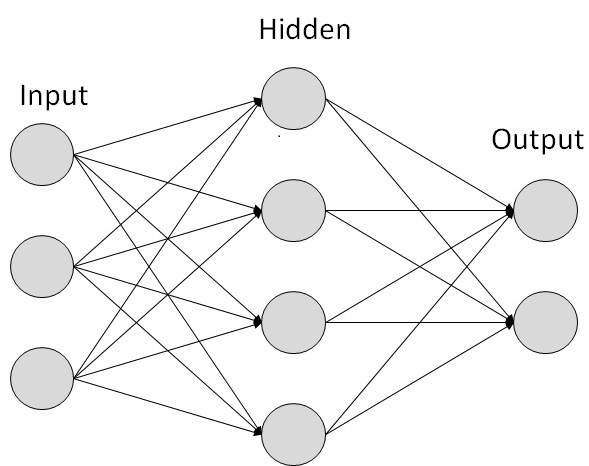
\includegraphics[width=10cm]{fcnn.jpg}
	\end{center}
	\caption{Fully-connected neural net.}
	\label{fig:fcnn}
\end{figure}

\begin{figure}
	\begin{center}
		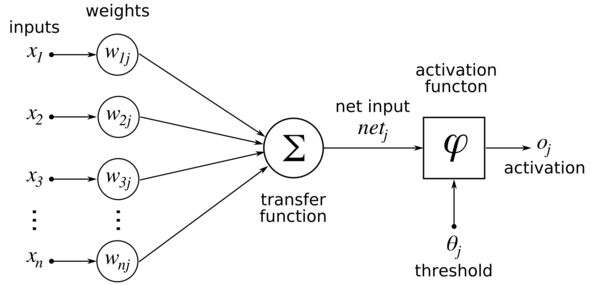
\includegraphics[width=10cm]{neuron.png}
	\end{center}
	\caption{Neuron.}
	\label{fig:neuron}
\end{figure}

\section{Solution}

\subsection{Related work}

There are several open source libraries for implementing neural networks, most of them are optimized for convolutional neural networks and deep learning networks. Some libraries which can be used are cuDNN\cite{cudnn} by NVidia, tensorflow\cite{tensorflow} and Caffe\cite{caffe}. This are huge libraries focusing mainly on deep learning but they can be used for fully-connected networks as well.

\subsection{Serial implementation}
The training of an MLP neural net consists in two basic phases: the feed-forward step when some input is given to the net which should flow through it and by the activation of the neurons some output is generated; the secondary step is the backpropagation step where the generated output is compared to the target output resulting in some kind of an error value. This error is backpropagated through the net calibrating the weights. 
The feed-forward step can be implemented as it follows:

\begin{verbatim}
Parameter: Layers (vector of layers), Neuron (vector of neurons 
in each layer), Inputs(vector of inputs), IN(number of inputs)
Variable: neuron (value of each neuron), i (value of each 
input), layer(value of each layer), sum(placeholder)

for each layer in Layers
  sum := 0
  for each neuron in Neurons
    for i := 0 to IN
      sum += weight[i] * Inputs[i]
    end for
  neuron.activation = activationFunction(sum)
  end for
end for
	
\end{verbatim} 

The backpropagation step is solved using gradient descent method. The chain rule of the gradient descent can be implemented as following:

\begin{verbatim}
Parameter: Layers (vector of layers), Neuron (vector of neurons 
in each layer), Outputs(vector of outputs), ON(number of outputs)
Deltas(vector of deltas)
Variable: neuron (value of each neuron), i (value of each 
input), layer(value of each layer)

for each layer in Layers
  for each neuron in Neurons
    for i := 0 to ON
      gradients[i] += Deltas[i] * 
        activationFunctionDerivative(Outputs[i])
    end for
  end for
end for
	
\end{verbatim}

For the output layer, the delta values can be calculated with a subtraction of the output value from the target value in case of every neuron. In case of hidden layers the delta value for every neuron in a layer is calculated by summing up the product of the weights and gradient values of every neuron from the following layer on which it has impact. 

\begin{verbatim}
Parameter: myNeuronIdx (the neuron for which we compute the delta
values), N (number of neurons in the nextLayer)
for i := 0 to N
  deltas[i] = weights[i][myNeuronIdx] * gradient[i]
end for
\end{verbatim}

After the gradients are computed, the last step is to update the weights in every layer. The weights are updated with this formula:

\begin{equation}
weight += trainRate * activatonRes * gradient + momentum * oldDelta
\end{equation} 

\subsection{Parallel implementation of the feed-forward step}
Every layer could have one ore more inputs. This inputs can be grouped together in a vector. 
\[ \left( \begin{array}{ccccc}
i_{0} & i_{1} & i_{2} & ... & i_{N} \end{array} \right)\] 
Because of the nature of the fully-connected layer, every neuron has to have a connection with every input. The weights of a neuron can be represented as a column in a matrix. We can create having the width the number of neurons present in the layer and the height being the number of the inputs. 
\[ \left( \begin{array}{ccccc}
W_{00} & W_{01} & W_{02} & ... & W_{0M} \\
W_{10} & W_{11} & W_{12} & ... & W_{1M} \\
... & ... & ... & ... & ... \\
W_{N0} & W_{N1} & W_{N2} & ... & W_{NM} \end{array} \right)\] 

Where: \\
N - number of inputs \\
M - number of neurons in the layer \\

In this case if we multiply the vector of inputs with the matrix of the weights, we get a result which applied to the activation function gives the output of the layer. Basically the feed-forward step of every layer can be done by solving a vector matrix multiplication. Using parallel programming this can be implemented with the usage of shared memory following a so called tiled approach. First of all we allocate two buffers in the shared memory, the first one is a single dimension array, the second one is a two-dimensional array. In the first buffer we will cache the input values, in the second array the weights are copied. Multiplying this arrays together we get a partial result. Next the remaining tiles are loaded into the shared memory. The partial results are summed up at the end. The final result will be a one-dimensional array of which values will be applied to the activation function. This step also is done when the results are gathered together.

\subsection{Parallel implementation of the backpropagation step}\
Each delta value can be individually calculated at the same time. They don't have cross-dependencies. For the output layer, the parallelization is simple, we start a big number of threads, every thread should calculate a single value. At the ending this values are copied to the global memory of the GPU. The parallel implementation for the hidden layer gradients has an inner loop which calculates sum. The simple solution for this is to have a loop in every thread. Because every thread will calculate the delta value using the same number of neurons, it is guaranteed that the threads wont encounter branching and none of the threads will introduce bottlenecks. Also, this sum can be calculated by using regression but this wont really have an impact if the number of neurons are not huge. Furthermore, this implies using dynamic parallelization which wont be achievable without proper hardware support.
Having the delta values already calculated the gradient values also can be easily computed launching a single kernel where every thread calculates a single gradient value. Finishing up this step, the update of the weights can be done following the same logic. 
It is important to know that computing the delta values, computing the gradients and updating the weights are steps that depend on each other. This excludes having them run in simultaneously. Even if we would be in the situation of having the independent steps, this would result in task parallelism for which is not advisable to use CUDA.

\subsection{Memory management - Naive approach}
The naive approach to do the parallelism of an MLP neural net would be that net is stored inside RAM memory. When the parallel kernels are executed, the necessary data will be transferred to the GPU memory. It turns out that this approach can massively slow down the training process because the RAM - VRAM communication is not negligible at all. The speed gain from the parallel sections is not comparable with the slow-downs occurring copying data.

\subsection{Memory management - Optimized approach}
The optimized approach is to allocate the memory at the beginning in the VRAM and use this memory until the training is completed. For this solution implementation of RAII (Resource acquisition is initialization) classes are the way to go. In the constructor of our net and layer class we allocate the needed memory and we will free up when the classes are destructed. This means we need to have enough GPU memory for keeping the entire net in it. Moreover, the training samples also have to be copied inside the GPU memory for a better speed gain and avoiding bottlenecks. In practice, the memory need for the training sample can exceed the memory space of the net. Using a modern GPU, the size of the memory should not be a problem, otherwise there are several methods for splitting up training samples and keeping only the necessary in the VRAM. 
We the memory is allocated, the CPU gets a pointer to it. This is very important looking back to the steps of the backpropagation. This way the CPU is the manager of what kernel should run at the specific moment. It also passes as an argument the pointer of the memory location which should be used.

\section{Benchmarks}
The input data used for benchmarks is the MNIST database\cite{mnist}. This contains 60000 images of handwritten digits. The size of every image is 28x28. 4 different neural nets were used for testing having the following topologies: Net1: layer1 - 128 neurons, layer2 - 128 neurons; Net2: layer1 - 128 neurons, layer2 - 128 neurons, layer3 - 128 neurons; Net3: layer1 - 1024 neurons, layer2 - 1024 neurons; Net4 - layer1 - 1024 neurons, layer2 - 1024 neurons, layer3 - 1024 neurons. Tests were done using the serial implementation and the parallel implementation for every net as well. The CPU used for testing is an intel I7 6700 clocked at 3.4 GHz, the GPU used for testing is an nVidia Geforce GTX1080 with 2560 CUDA cores. For each net the average training iteration time was measured. In an iteration the training of a single image is done. This image data is fed 10 times to the net and then the upcoming image is taken. An epoch is passed when every iteration is finished. The training lasts multiple epochs. The results are displayed in milliseconds and they are the following:

\begin{center}
\begin{tabular}{| l | l | l | l |}
\hline
Net & Topology & CPU & GPU \\
\hline
Net1 & 128 - 128 & 15 ms & 16 ms  \\
Net2 & 128 - 128 - 128 & 18 ms & 15 ms  \\
Net3 & 1024 - 1024 & 150 ms & 38 ms  \\
Net4 & 1024 - 1024 - 1024 & 615 ms & 72 ms  \\
\hline
\end{tabular}
\end{center}

\begin{figure}[!htbp]
	\begin{center}
		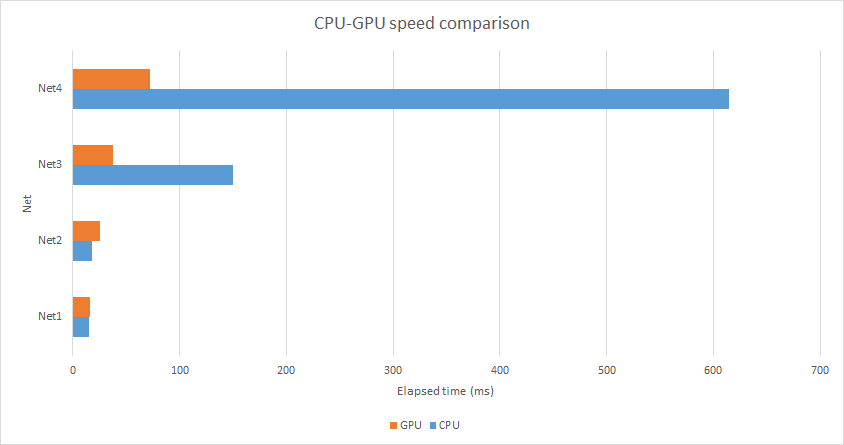
\includegraphics[width=15cm]{chart.png}
	\end{center}
	\caption{CPU-GPU speed comparison}
	\label{fig:chart}
\end{figure}

We can observe that the CPU has the faster times when then net is relatively small. Also it take a considerable advantage when the number of serial operations increase, having more layers for which to calculate the outputs. The GPU takes serious advantage when the number of neurons increase. Having more neurons increases the number of the parallel operations, reaching a speed-up of 8.54 at the last net. As the numbers of neurons increase per layer, the more effective the parallel algorithm is.  

\section{Conclusion}

I conclusion we can state that we were able to give a parallel implementation for the MLP neural net. We were able to optimize the given solution in an way to avoid data transfers between the RAM and the VRAM in the training process. Also we have demonstrated that the GPU takes a serious lead when dealing with data parallelism compared to the CPU. 

\section{References}

\printbibliography

\end{document}



